\documentclass{beamer}
\usepackage[english]{babel}
\usepackage{calc}
\usepackage[absolute,overlay]{textpos}
\mode<presentation>{\usetheme{tud}}

\title[Mid-term Presentation]{Leveraging VLC for energy }
\subtitle{disaggregation in Smart Buildings}
\institute[TU Delft]{Delft University of Technology}
\author{Johnny Verhoeff}
\date{\today}

% Insert frame before each subsection (requires 2 latex runs)
\AtBeginSubsection[] {
	\begin{frame}<beamer>\frametitle{\titleSubsec}
		\tableofcontents[currentsection,currentsubsection]  % Generation of the Table of Contents
	\end{frame}
}
% Define the title of each inserted pre-subsection frame
\newcommand*\titleSubsec{Next Subsection}
% Define the title of the "Table of Contents" frame
\newcommand*\titleTOC{Outline}

% define a symbol which can be removed if you don't need it
\newcommand{\field}[1]{\mathbb{#1}}
\newcommand{\Zset}{\field{Z}}

\begin{document} {
	% remove the next line if you don't want a background image
	\usebackgroundtemplate{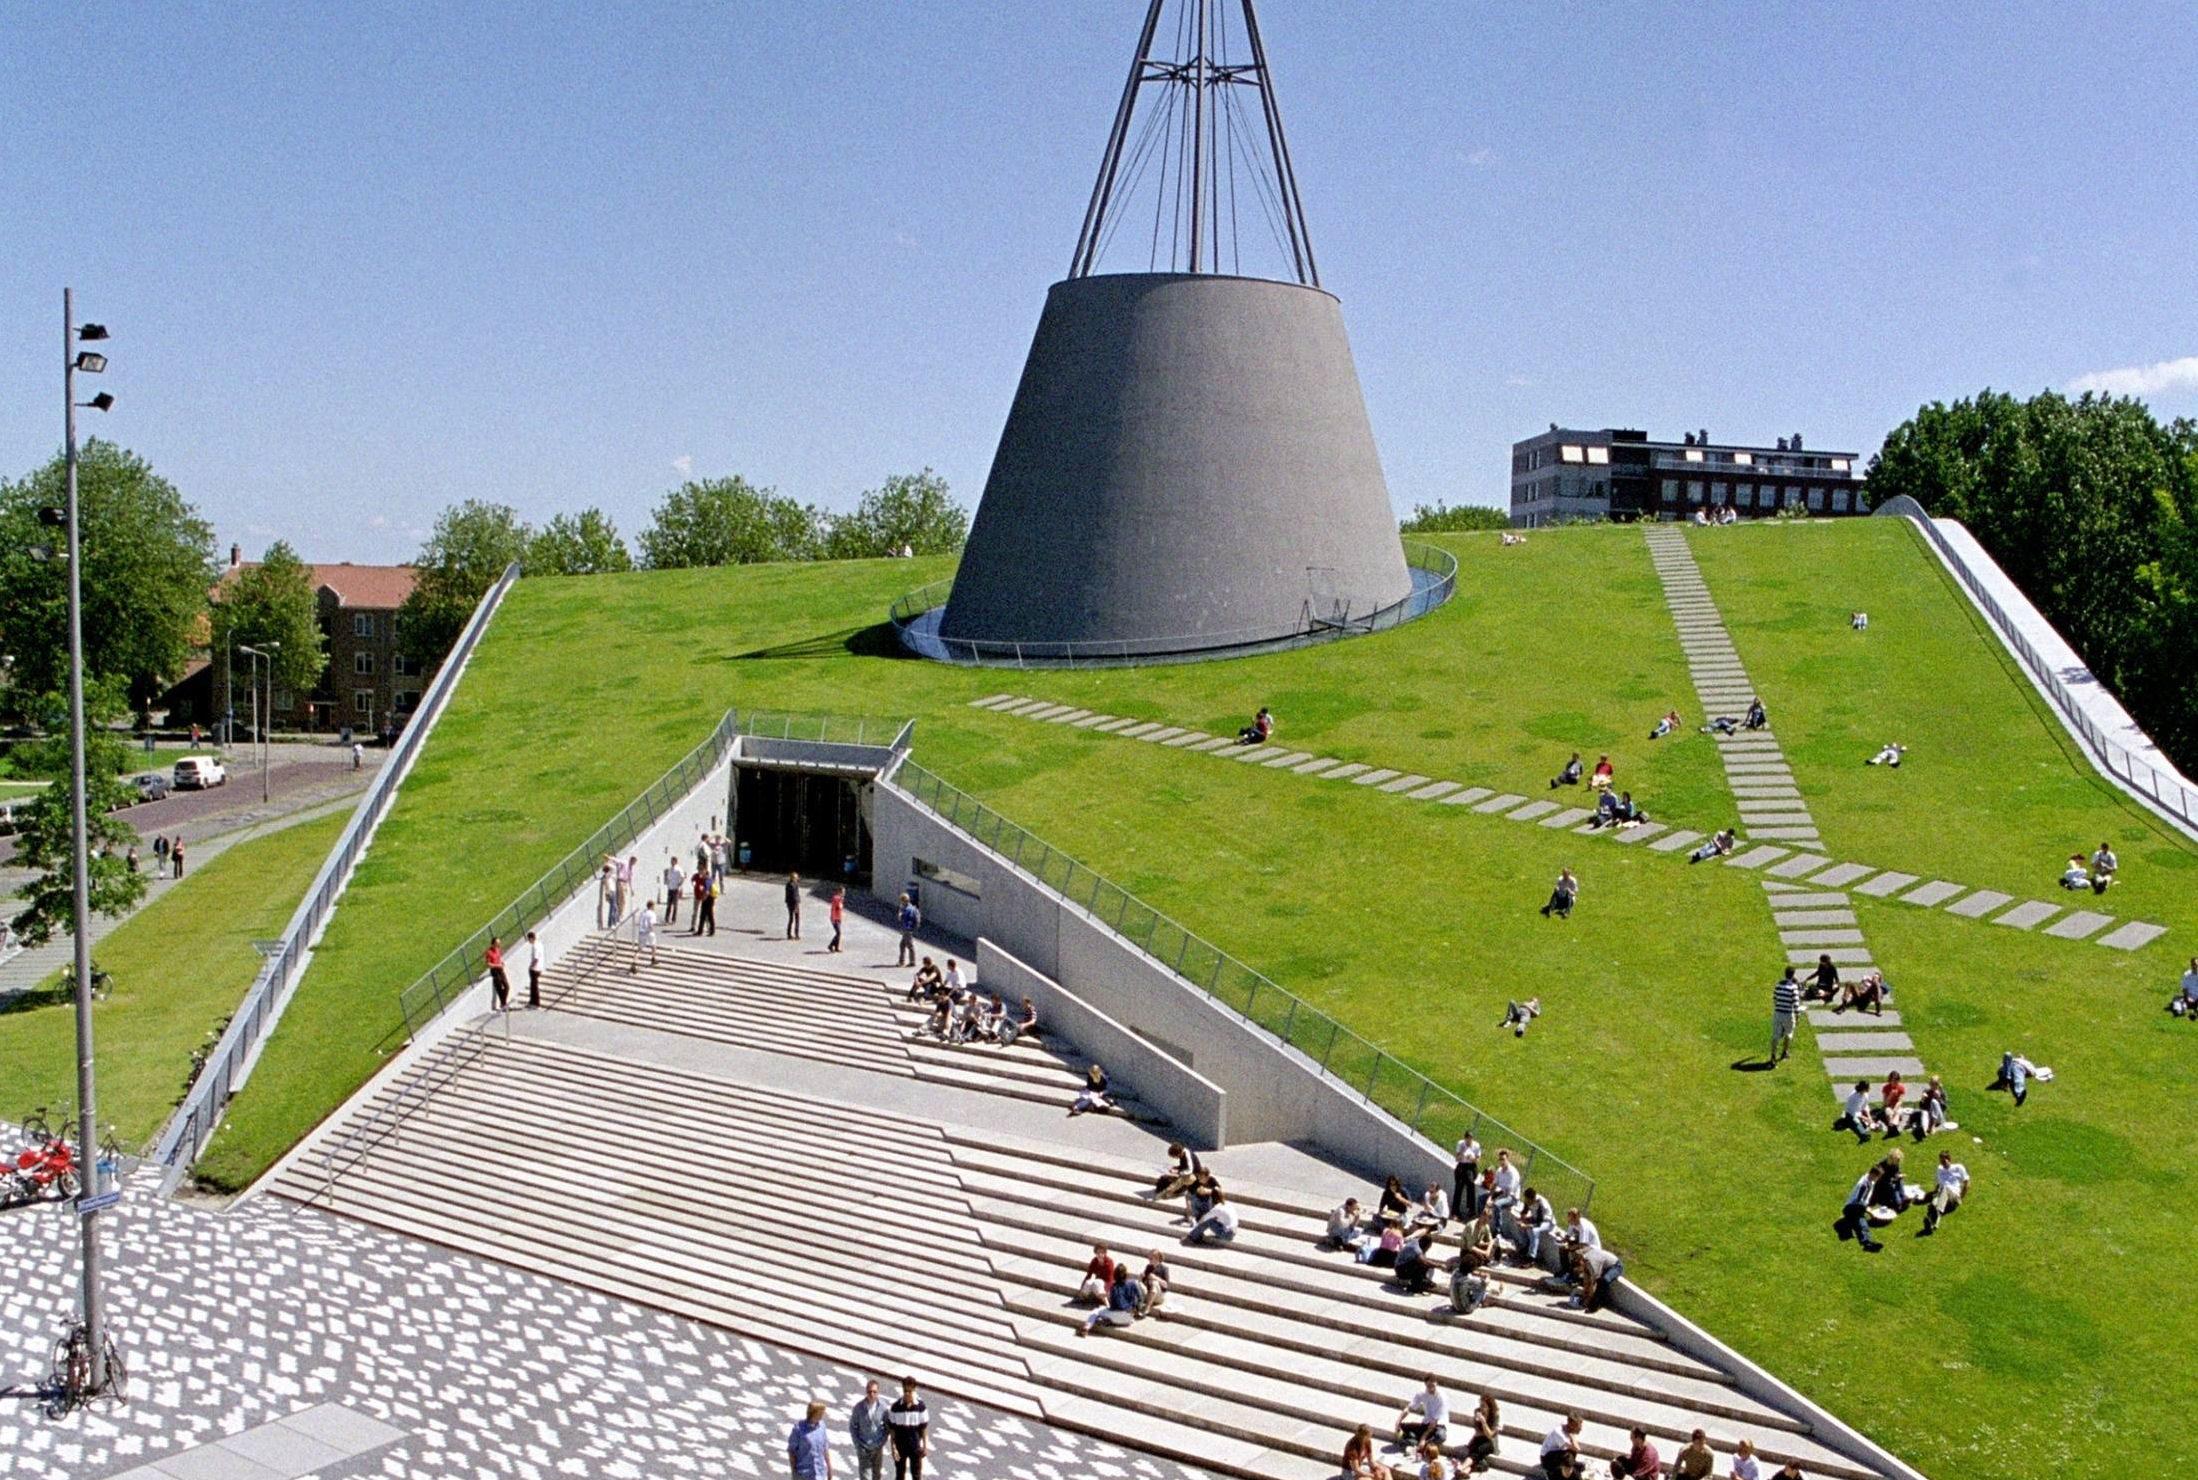
\includegraphics[width=\paperwidth,height=\paperheight]{images/background-titlepage.jpg}}%
	\setbeamertemplate{footline}{\usebeamertemplate*{minimal footline}}
	\frame{\titlepage}
}

\beamertemplatenavigationsymbolsempty
%\setbeamertemplate{navigation symbols}{}

%{\setbeamertemplate{footline}{\usebeamertemplate*{minimal footline}}
%\begin{frame}\frametitle{\titleTOC}
%	\tableofcontents
%\end{frame}
%}

%\section{First Section}
%\subsection{Section 1 - Subsection 1}


	%intro
	\begin{frame}\frametitle{TITLE}
		Energy disaggregation successful for refrigerators and HVAC because they have  unique signature
	\end{frame}

	\begin{frame}\frametitle{TITLE}
		Lighting doesn't have unique signature but is important because X \% of energy is used for lighting
	\end{frame}

	\begin{frame}\frametitle{TITLE}
		Use VLC to modulate lights and give lighting an unique signature through the current they draw
	\end{frame}

	\begin{frame}\frametitle{TITLE}
		Easiest way to use VLC is with OOK, lighting currents will be superimposed
	\end{frame}


	%hardware

	\begin{frame}\frametitle{TITLE}
		DC: use current source per LED for constant and flat current curve, with nice superimposition results
	\end{frame}

	\begin{frame}\frametitle{TITLE}
		AC is not constant, LED require certain amount of voltage
	\end{frame}

	\begin{frame}\frametitle{TITLE}
		Detection circuit for a certain amount of voltage for LEDs and current source for constant and flat current curve, with nice superimposition results
	\end{frame}

	\begin{frame}\frametitle{TITLE}
		DC: use burden resistor with output to adc to measure DC current
	\end{frame}

	\begin{frame}\frametitle{TITLE}
		AC: hall effect too noisy, so also use burden resistor: will produce + and - voltage
	\end{frame}

	\begin{frame}\frametitle{TITLE}
		AC: burden resistor will produce + and - voltage so add half of adc vcc and then to ADC
	\end{frame}




	%cdma

	\begin{frame}\frametitle{TITLE}
		All LEDs are basically transmitters on same freq. and same time.
	\end{frame}

	\begin{frame}\frametitle{TITLE}
		Therefor TDM and FDM are out and CDM is used
	\end{frame}

	\begin{frame}\frametitle{TITLE}
		Concept of correlation: auto and cross
	\end{frame}

	\begin{frame}\frametitle{TITLE}
		Want low cross correlation with all time shifts and high autocorr. at zero time shift and low autocorr at all other time shifts.
	\end{frame}

	\begin{frame}\frametitle{TITLE}
		comparison of orth. pn and gold
	\end{frame}



	% testbed

	\begin{frame}\frametitle{TITLE}
		DC test bed 6 individual LEDs
	\end{frame}

	\begin{frame}\frametitle{TITLE}
		AC test bed 3 individual commercial LEDs
	\end{frame}

	\begin{frame}\frametitle{TITLE}
		Correlation results with contious method DC
	\end{frame}

	\begin{frame}\frametitle{TITLE}
		Correlation results with contious method AC
	\end{frame}





	\begin{frame}\frametitle{TITLE}
		Something with scalabity ??
	\end{frame}


	\begin{frame}\frametitle{TITLE}
		Conclusion ... ? ? 
	\end{frame}











\end{document}
